\documentclass[11pt,a4paper]{extarticle}
\usepackage[utf8]{inputenc}
\usepackage[T1]{fontenc}
\usepackage[hidelinks]{hyperref} 
\usepackage[russian,english]{babel}
\usepackage{amsthm}
\usepackage{listings}
\usepackage{amsmath}
\usepackage{amsfonts}
\usepackage{amssymb}
\usepackage{xcolor,colortbl}
\usepackage{graphicx}
\usepackage{subcaption}
\usepackage{fullpage}
\usepackage[nottoc,numbib]{tocbibind}

\definecolor{Gray}{gray}{0.95}
\definecolor{Red}{rgb}{0.80,0.5,0.5}
\definecolor{Green}{rgb}{0.6,0.8,0.6}

\newenvironment{compactlist}{
\begin{list}{{$\bullet$}}{
\setlength\partopsep{0pt}
\setlength\parskip{0pt}
\setlength\parsep{0pt}
\setlength\topsep{0pt}
\setlength\itemsep{0pt}
}}{
\end{list}
}

\begin{document}
\selectlanguage{russian}
	\begin{titlepage}
		\begin{centering}
			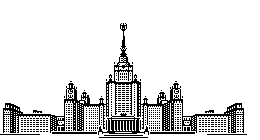
\includegraphics{msu}\\
				\large{
					\textbf{Московский государственный университет имени М.\ В. Ломоносова}\\
					Факультет вычислительной математики и кибернетики\\
					Кафедра автоматизации систем вычислительных комплексов\\[4cm]
				}
				\Large{
					Курсовая работа\\[0.5cm]
				}
				\Large{
					\textbf{Декомпозиция невыпуклых объектов\\ для решения задач обнаружения пересечений}\\					
					% \textbf{Convex Decomposition in Collision Detection}\\
				}
				\rule[0.3cm]{14cm}{0.02cm}\\[3cm]
		\end{centering}
		\begin{flushright}
			\large{
			Гончаренко Дмитрий Александрович\\
			320 группа \\

			\textbf{Научный руководитель:} с.н.с. Игнатенко А.В.\\
			}
		\end{flushright}
		\begin{center}
			\vfill 
			\large{
				Москва, 2018
			}
		\end{center}
	\end{titlepage}

	\begin{abstract}
		В данной работе поднимается актуальная проблема в компьютерной графике -- \emph{выпуклое разбиение 
		фигур}\footnote{здесь и далее \textbf{выпуклое разбиение} - разбиение произвольной фигуры на только выпуклые части}, 
		использующееся для дальнейшего поиска пересечений объекта в сцене. 
		Рассматриваются алгоритмы декомпозиции и методы решения поставленной задачи, в том числе иерархия ограничивающих объемов.
		Реализована декомпозиция сложнополигональных объектов на основе библиотеки HACD на языке C++. 
		Проведена сравнительная характеристика точного и приблизительного разбиений на примере 14 невыпуклых объектов.
	\end{abstract}
	
	\newpage
	\tableofcontents
	
	\newpage

	\section{Введение}
	Компьютерная графика все сильнее проникает в науку, медицину, сферу развлечений.
	Поиск столкновений, вычисление расстояний и глубины проникновения объектов - задачи, остающееся актуальноми уже не первый десяток лет. 
	Появление GPU, многопоточной структуры для массивных параллельных вычислений, стало, несомненно, прорывом для трехменой графики в целом.
	Сейчас повсеместно используются графические процессоры для ускорения вычислений объемных объектов.
	CPU и комбинированные решения GPU и CPU используются для достижения наилучшей точности в обработке графической информации.
	
	В своей работе я рассматриваю задачи, возникающие при попытке обнаружения точного пересечения объектов.
	Одной из таких задач является проблема поиска столкновений нетривиальных фигур.
	Сложность вычисления в случае невыпуклых объектов резко возрастает. 
	Популярным и наиболее действенным решением на текущий момент считается разбиение (декомпозиция) фигуры на выпуклые части, что значительно упрощает процесс обнаружения пересечений.

	Ниже описаны основные задачи, с которыми можно столкнуться при изучении поставленного вопроса.
	Такие как поиск оптимальных алгоритмов, NP-сложность разбиения трехмерных объектов, точная декомпозиция многогранников (ECD) и выбор стратегий иерархии ограничивающих объемов.
	
	\section{Предметная область}
		\subsection{Понятие выпуклости}
			Для начала, введем общее понятие выпуклости.\\
			\textbf{Выпуклым} называется множество, в котором все точки отрезка, образуемого любыми двумя точками данного множества, также принадлежат данному множеству.\\
			\textbf{Выпуклой оболочкой (convex hull)} множества $X$ называется наименьшее выпуклое множество, содержащее $X$.
			\begin{figure}[ht]
				\centering
				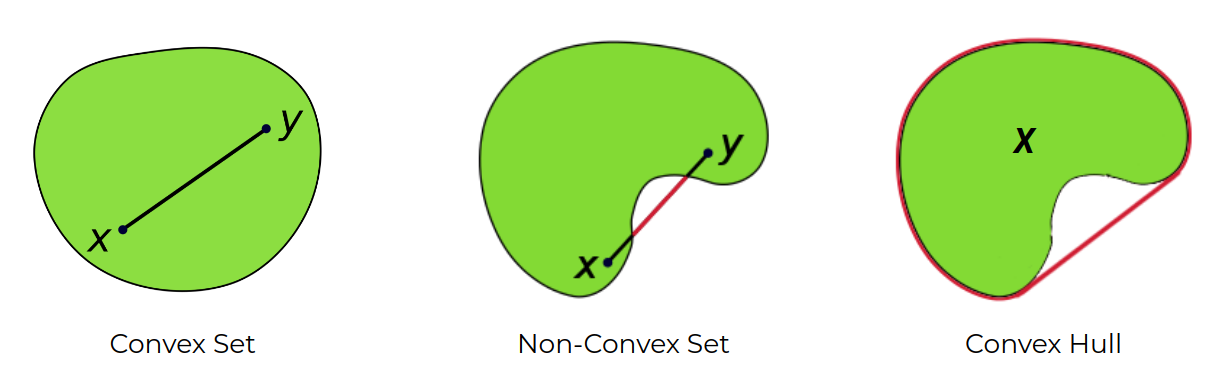
\includegraphics[width=\textwidth]{convexes}
			\end{figure}
		\newpage
		\subsection{Проверка на выпуклость}
			Для того чтобы определить, является ли выбранный многоугольник или многогранник выпуклыми, используют различные алгоритмы. Рассмотрим некоторые из них.
			\paragraph{Многоугольник.} На плоскости используют следующие методы определения выпуклости:
			\begin{enumerate}
				\item Для каждого ребра вычислить, лежат ли все несмежные вершины строго по одну сторону от выбранного ребра. Сложность $O(n^2)$. (см.\,рис\,\ref{con_polygon})
				\item Для каждого внутреннего угла проверить, меньше ли он $180^{\circ}$. Сложность $O(n)$. Работает только для фигур без самопересечений (пр. ''звезда'' - невыпуклая).
				\item Проделать циклический путь по всем смежным вершинам. Должно быть только две смены направления.  
			\end{enumerate}

			\begin{figure}[ht]
				\centering
				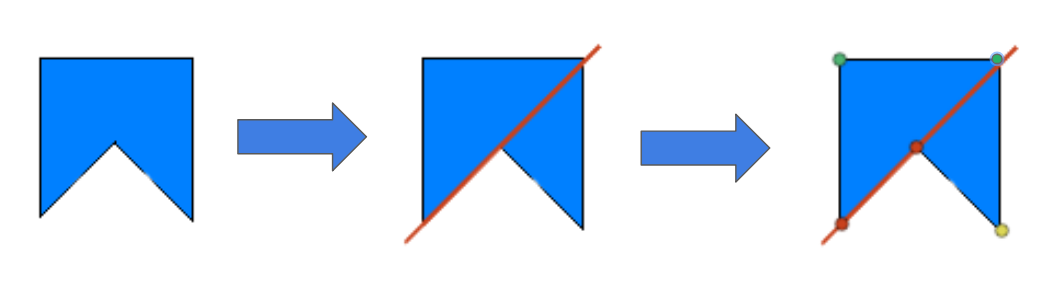
\includegraphics[width=0.8\textwidth]{con_polygon}
				\caption{Невыпуклый многоугольник с опорной прямой (красная линия)}
				\label{con_polygon}				
			\end{figure}
			\paragraph{Многогранник.} В трехмерном случае выделяются следующие алгоритмы:
			\begin{enumerate}
				\item Для каждой грани вычислить, лежать ли все несмежные вершины строго по одну сторону от этой грани. Сложность $O(n^2)$. (см.\,рис.\,\ref{con_polyhedra})
				\item Для каждой грани F многогранника P вычислить центроид\footnote{центроид (или барицентр) - центр масс} С. Для каждой соседней грани G проверить, лежит ли их C за опорной плоскостью G. Если для всех граней это выполняется, то фигура предполагается выпуклой, иначе она является невыпуклой. Сложность $O(n)$.
			\end{enumerate}	
			\begin{figure}[ht]
				\centering
				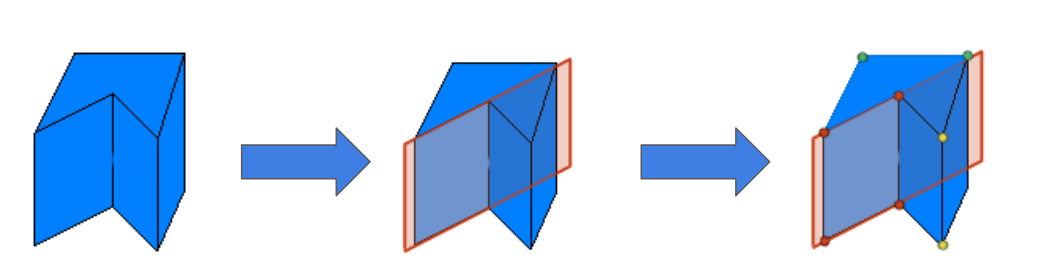
\includegraphics[width=0.8\textwidth]{con_polyhedra}
				\caption{Невыпуклый многогранник с опорной плоскостью (красный прямоугольник)}
				\label{con_polyhedra}
			\end{figure}
	
	
	\newpage

	\section{Задача}
		\subsection{Цели работы}
			В точном обнаружении пересечений невыпуклых фигур возникают проблемы падения скорости и возрастания сложности вычислений.
			С этой проблемой справляются разбиение фигуры на упрощенные выпуклые части и иерархия ограничивающих объемов.
			В свою очередь задачи оптимального выпуклого разбиения фигур в трехмерном пространстве являются нетривиальными.
			Целью работы является исследование алгоритмов выпуклого разбиения и реализация выбранного метода на C++. 
		\subsection{Постановка задачи}
			\begin{enumerate}
				\setlength\partopsep{0pt}
				\setlength\parskip{0pt}
				\setlength\parsep{0pt}
				\setlength\topsep{0pt}
				\setlength\itemsep{0pt}
				\item Рассмотреть основные методы декомпозиции, такие как триангуляция Делоне, тетрайдаризация, методы точного и приблизительного разбиения.
				\item Исследовать NP-полную задачу о невозможности разбиения невыпуклых многогранников.
				\item Привести возможные алгоритмы ее решения.
				\item Сравнить стратегии построения иерархий ограничивающих объемов.
				\item Реализовать выбранный алгоритм разбиения.
			\end{enumerate}
	
	\section{Алгоритмы разбиения}
		
		\subsection{Триангуляция на плоскости}
			\textbf{Триангуляция --} процесс/результат разбиения геометрической фигуры на симплексы\footnote{Симплекс (n-мерный тетраэдр) -- фигура, являющаяся n-мерным обобщением треугольника.}.
			Одним из алгоритмов триангуляции многоугольника является \emph{алгоритм обрезки ушей$^{\footnotesize{\ref{ears}}}$} (рис.\,\ref{earcut}). 
			Сформулируем соответсвующую теорему.
			
			\newtheoremstyle{break}
			{}{}%
			{\itshape}{}%
			{\bfseries}{}%
			{\newline}{}%
			\theoremstyle{break}
			\newtheorem*{theorem1}{Теорема Мейстерса (о двух ушах)\footnote{\label{ears}Ушами многоугольника называют треугольники, две стороны каждого из которых являются сторонами многоугольника, а третья лежит полностью внутри него.}}			
			\begin{theorem1}
				Любой простой n-угольный полигон с n > 3 имеет как минимум два уха.
			\end{theorem1}
			\noindent
			\textbf{Cуть алгоритма}\;\;
			Находится очередное ухо и отрезается от многоугольника. После этого операция повторно применяется к оставшемуся многоугольнику до тех пор, пока не останется один треугольник.	
			рис.\,\ref{earcut} 
			\begin{figure}[ht]
				\centering
				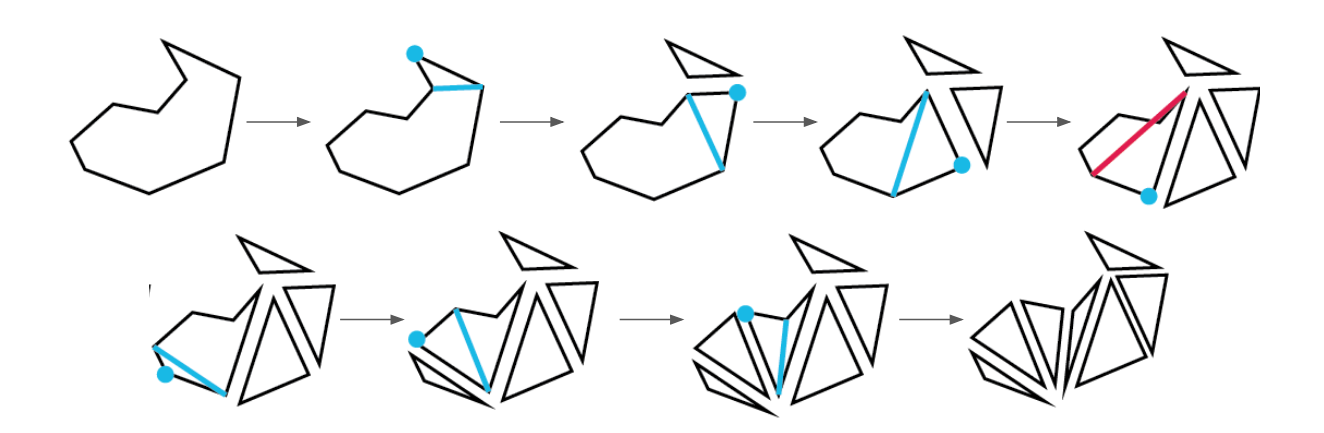
\includegraphics[width=0.9\textwidth]{earcut}
				\caption{Алгоритм отрезания ушей (Ear Cutting Algorithm)}
				\label{earcut}
			\end{figure}
			
			\newpage
			\paragraph{Преимущества и недостатки}
			Этот способ работает только для многоугольников без дырок. Он прост в реализации, но медленнее, чем некоторые другие алгоритмы. 
			Алгоритм работает за время $O(n^{2})$. Результирующая декомпозиция не является оптимальной.\\
			\textbf{Оптимизация}\:\:
			Не вызывает сомнения, что разбиение полученное методом отрезания ушей может быть выполнено не единственным способом.
			Еще в прошлом веке Хертелем и Мелхорном был придуман оптимизирующий \emph{алгоритм удаления возможных диагоналей}.
			Его суть заключается в следующем: в процессе триангуляции удаляются все возможные диагонали, убрав которые не появляются невыпуклые вершины. 
			Другими словами, полученная декомпозиция остается выпуклой.
			рис.\,\ref{hmalg}
			\begin{figure}[ht]
				\centering
				\begin{subfigure}[ht]{1in}
					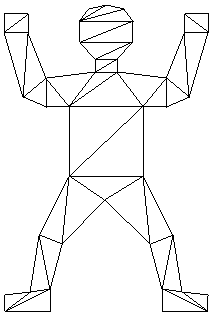
\includegraphics[width=0.9\textwidth]{hm1}
					\caption{}
				\end{subfigure}
				\hspace{0.7cm}
				\LARGE{$\longrightarrow$}
				\hspace{0.7cm}
				\begin{subfigure}[ht]{1in}				
					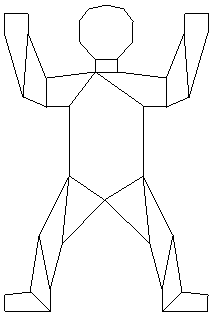
\includegraphics[width=0.9\textwidth]{hm2}
					\caption{}
				\end{subfigure}
				\caption{Алгоритм Hertel-Mehlhorn. (а) - триангуляция, (b) - после работы алгоритма}				
				\label{hmalg}
			\end{figure}\\
			Предложенный алгоритм можно встроить непосредственно в процесс триангуляции.
			Для этого достаточно на каждом шаге проверять, возможно ли объеденить только что отрезанное ухо с предыдущим многоугольником.
			Если да - объединять с предыдущим, иначе - предыдущим многоугольником становится отрезанный треугольник \cite{RTCD}.
			Как показывает эвристика, полученная триангуляция методом удаления лишних диагоналей близка к оптимальной.
			
			\subsubsection{Триангуляция фигур с отверстиями}
				Из предыдущего параграфа стало ясно, что алгоритм отрезания ушей перестает функционировать в случае присутствия в геометрии .
				Для разрешения этой ситуации потребуется или дополнительное разбиение фигуры на несколько монотонных\footnote{Многоугольник называется \textbf{монотонным}, если его граничная ломаная имеет не более двух точек пересечения с прямой, перпендикулярной данной.} частей,
				или вырезание из многоугольника канала нулевой ширины с перенумерацией вершин (рис.\,\ref{cutholes}).
				\begin{figure}[ht]
					\centering
					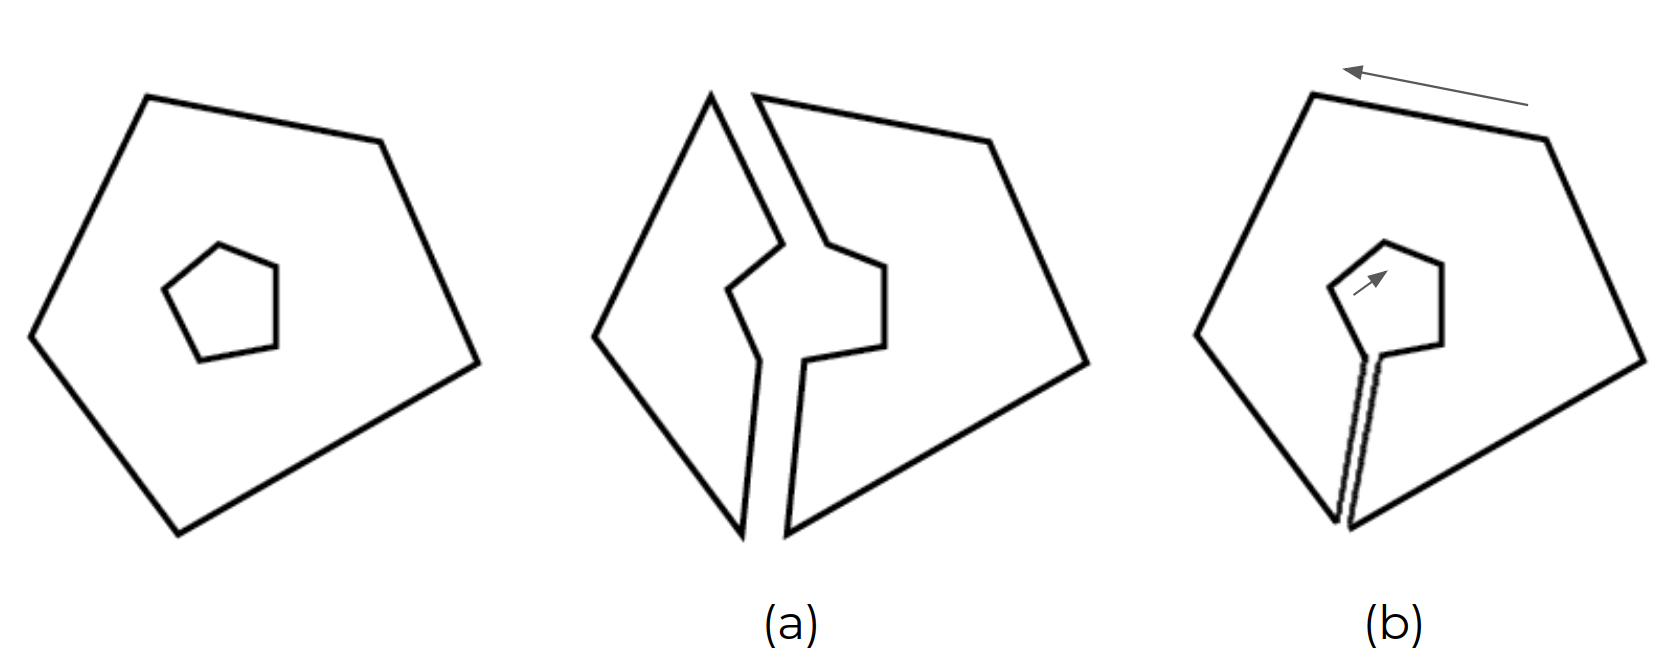
\includegraphics[width=0.8\textwidth]{cutholes}
					\caption{(a) - декомпозиция полигона на монотонные части,
							 (b) - “канал” нулевой ширины}
					\label{cutholes}
				\end{figure}

			\subsubsection{Триангуляция Делоне} 
				\textbf{Триангуляция Делоне --} триангуляция для заданного множества точек S на плоскости, при которой для любого треугольника все точки из S за исключением точек, являющихся его вершинами, лежат вне окружности, описанной вокруг треугольника.
				Из каждой точки порождается окружность, проходящая через две ближайшие точки (рис.\,\ref{delone}).\\
				Интересаня \href{https://github.com/snorpey/triangulate-image}{реализация метода} на изображениях представлена на рис. \ref{msu_delone}. \cite{img_delone}
				\begin{figure}[ht]
					\centering
					\begin{subfigure}[ht]{2in}
						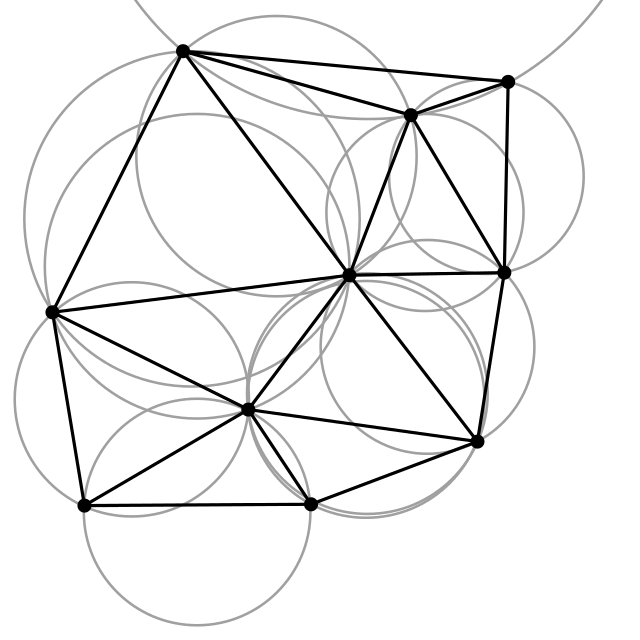
\includegraphics[width=\textwidth]{delone}	
						\caption{}
						\label{delone}	
					\end{subfigure}
					\begin{subfigure}[ht]{3in}
						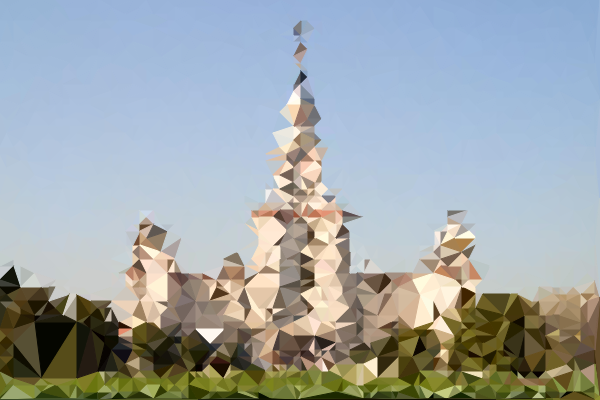
\includegraphics[width=\textwidth]{msu_delone}	
						\caption{}	
						\label{msu_delone}
					\end{subfigure}
					\caption{(a) - пример триангуляции Делоне, (b) - \href{https://github.com/snorpey/triangulate-image}{триангуляция картинки Делоне}}	
				\end{figure}\\
				\textbf{Свойства}\:\: Триангуляция Делоне -- 
				\begin{compactlist}
					\item взаимно однозначно соответствует диаграмме Вороного для того же множества точек.
					\item единственна, если никакие четыре точки не лежат на одной окружности.
					\item максимизирует минимальный угол среди всех углов всех построенных треугольников, тем самым избегаются «тонкие» треугольники.
					\item максимизирует сумму радиусов вписанных шаров.
					\item минимизирует дискретный функционал Дирихле.
					\item минимизирует максимальный радиус минимального объемлющего шара.
					\item на плоскости обладает минимальной суммой радиусов окружностей, описанных около треугольников, среди всех возможных триангуляций.\\
				\end{compactlist}
				\textbf{Алгоритм}\:\: Задача о нахождении триангуляции Делоне множества точек в d-мерном Евклидовом пространстве может быть сведена к задаче поиска выпуклой оболочки этого множества точек в (d+1)-мерном пространстве.
				Для этого необходимо каждой точке $p$ ввести дополнительную координату $|p|^2$.
				Возвращаясь к пространсву предыдущей размерности нужно удалить последнюю координату. 
				В связи с уникальностью выпуклой оболочки, триангуляция тоже будет уникальной (рис.\,\ref{lift_delone}).
				\href{https://github.com/jmlien/cshape2d}{Реализация на github} \cite{cshape2d}.
				\begin{figure}[ht]
					\centering
					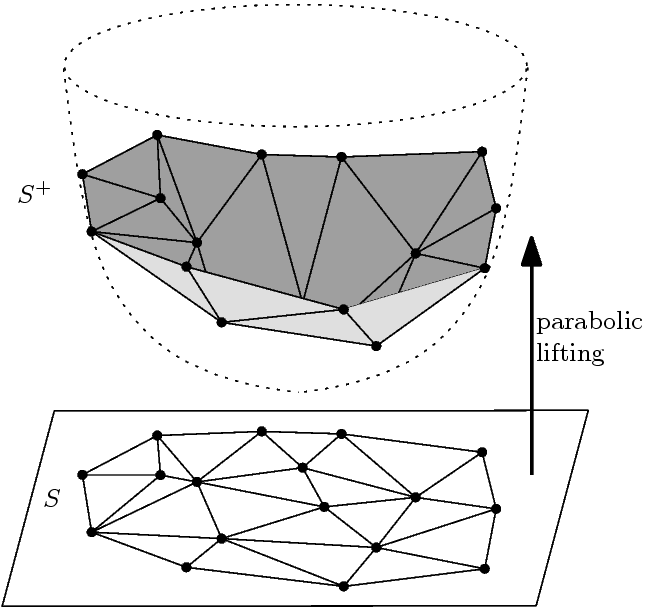
\includegraphics[width=0.24\textwidth]{lift_delone}
					\caption{Триангуляция Делануа через выпуклую оболочку}
					\label{lift_delone}
				\end{figure}
			
		\subsection{Трехмерная декомпозиция}
			В отличие от разбиения многоугольников, рассмотренного выше, не каждую фигуру в трехмерном пространстве можно триангулировать тетрайдерами без введения вспомогательных условий.
			Примером может послужить \emph{скрученная призма} -- невыпуклый призматический многогранник, полученный из однородной $q$-угольной путём деления боковых граней диагональю и вращения верхнего основания,
			обычно на угол $\pi / q$ радиан, в направлении, при котором стороны становятся вогнутыми (рис.\,\ref{shonhard}).
			Скрученная призма не может быть разбита на тетраэдры без введения новых вершин.
			\subsubsection{NP-полная задача разбиения невыпуклых многогранников}
				Скрученная призма с параметром $q=3$ называется \emph{многогранником Шёнхардта} (рис.\,\ref{shonhard}).
				На его основе было доказано, что триангуляция невыпуклого многогранника относится к классу NP-полных задач. 
				В свою очередь задача о минимальном разбиении выпуклого многогранника относится к классу NP-сложных задач \cite{RupSei92}.
				\begin{figure}[ht]
					\centering
					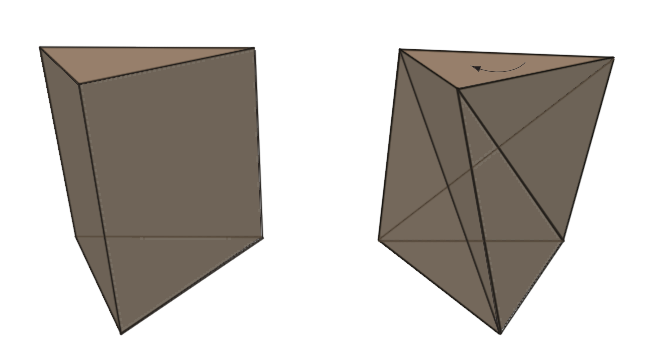
\includegraphics[width=0.65\textwidth]{shonhard}
					\caption{Многогранник Шёнхардта \\(невозможно триангулировать)}
					\label{shonhard}
				\end{figure}
				\begin{table}[ht]
					\centering
					\begin{tabular}{|p{0.22\textwidth}|p{0.45\textwidth}|p{0.25\textwidth}|}
					\hline
					\rowcolor{Red}
					\multicolumn{3}{|l|}{\textbf{Проблема}} \\
					\hline
					\rowcolor{Gray}
					\multicolumn{3}{|l|}{Невозможность триангуляции невыпуклого многогранника} \\
					\hline
					\rowcolor{Green}
					\textbf{Решение} & \textbf{Описание} & \textbf{Недостатки} \\
					\hline
					\rowcolor{Gray}						
					& &\\
					\rowcolor{Gray}
					Точки Штейнера & Ввести дополнительные точки разбиения вне объекта & Поиск расположения \\
					\rowcolor{Gray}
					& &\\\hline
					\rowcolor{Gray}
					& &\\
					\rowcolor{Gray}						
					Полигональный суп & Представить объект, в виде набора полигонов & Потеря информации	\\
					\rowcolor{Gray}
					& &\\\hline
					\rowcolor{Gray}
					& &\\
					\rowcolor{Gray}												
					CSG объекты & Использовать технологию Constructive Solid Geometry (см.\,рис.\,\ref{csg}) & Численная неточность \\
					\rowcolor{Gray}
					& &\\\hline
					
					\end{tabular}
				\end{table}\\
				\newpage
				\noindent
				Конструктивная блочная геометрия (CSG) является одним из возможных способом моделирования в трёхмерной графике. Она позволяет создать сложную сцену или объект с помощью битовых операций, комбинируя несколько иных упрощенных объектов
				(см.\,рис.\,\ref{csg}).
				\begin{figure}[ht]
					\centering
					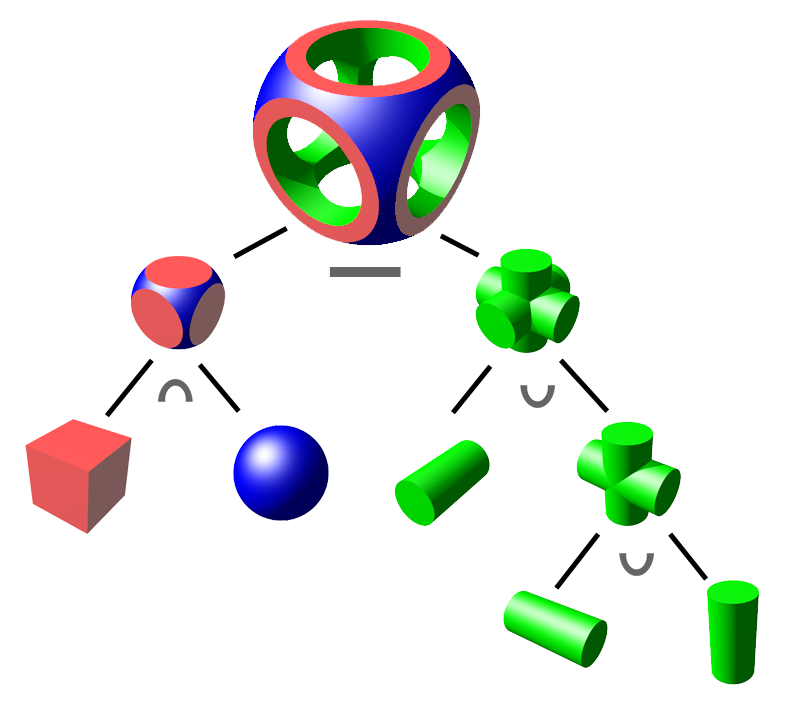
\includegraphics[width=0.5\textwidth]{csg}
					\caption{Пример КБГ. Двоичное дерево, где “листья” -- это объекты, а “узлы” -- операции}
					\label{csg}
				\end{figure} 
				
		\subsection{Точное и приблизительное разбиения}
			В некоторых ситуациях при декомпозиции сложных моделей, можно сильно сэкономить на вычислительных ресурсах, если вместо \emph{точного разбиения} считать \emph{приближенное}. 
			Во многих задачах такой подход, помимо увеличения эффективности и удобного иерархического представления, даст результат, не превышающий пределы допустимой точности \cite{JMLien06}.\\
			\begin{figure}[ht]
				\centering
				\begin{subfigure}{2in}
					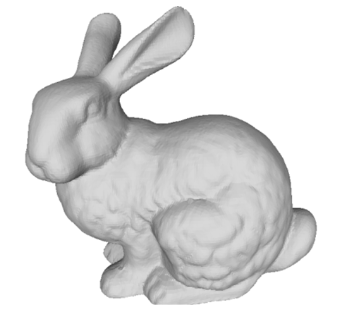
\includegraphics[width=0.8\textwidth]{acd1}					
					\caption*{исходная модель}
				\end{subfigure}
				\begin{subfigure}{2in}
					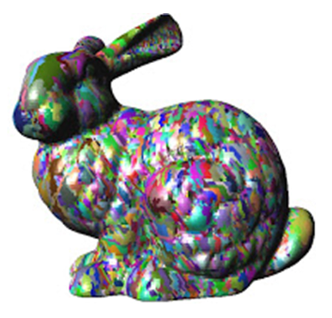
\includegraphics[width=0.8\textwidth]{acd2}					
					\caption*{7611 частей}
				\end{subfigure}
				\begin{subfigure}{2in}
					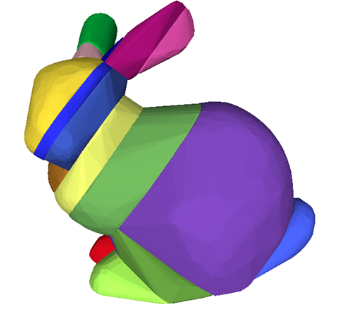
\includegraphics[width=0.8\textwidth]{acd3}					
					\caption*{20 частей}
				\end{subfigure}
				\caption{Точное и приближенное выпуклое разбиение}
			\end{figure}
			\begin{equation*}
				\begin{array}{ll}
					\text{Введем понятие \emph{меры вогнутости}.} \\
					\text{Декомпозиция многогранника:}&D(P) = \{ P_i\;|\;\cup_iP_i = P\;and\;\forall_{i\neq j}P_i\cap P_j = \emptyset \}\\
					\text{Мера вогнутости многогранника P:}&convave(P) = max_{x\in \partial P}\{concave(x)\}\\
					\text{Приближенная декомпозиция P:}&ACD_\tau(P) = \{P_i\;|\;P_i \in D(P)\;and\;concave(P_i) \leq \tau\}\\
					\text{Точная декомпозиция P:}& ECD(P) = ACD_0(P)
				\end{array}
			\end{equation*}
			\newpage
			\noindent
			Обозначим через $H_p$ выпуклую оболочку фигуры $P$.\\
			\textbf{Вогнутость (concavity)} $P$ можно измерить как расстояние от точки $x$ многогранника $P$ до $H_p$.
			Определим следующие вспомогательные понятия:\\
			\textbf{Мост (bridge)} -- выпуклая оболочка граней, соединяющих несмежные вершины границы многогранника $\partial P$.\\
			\textbf{Карман (pocket)} -- часть границы $\partial P$ которая не находится на выпуклой оболочки границы $\partial H_p$.\\
			\begin{figure}[ht]
				\centering
				\begin{subfigure}{2in}
					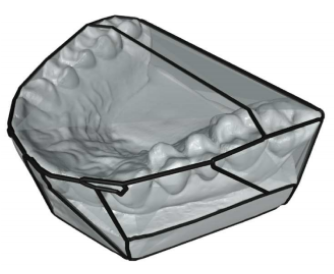
\includegraphics[width=0.8\textwidth]{teeth1}					
					\caption*{мосты}
				\end{subfigure}
				\begin{subfigure}{2in}
					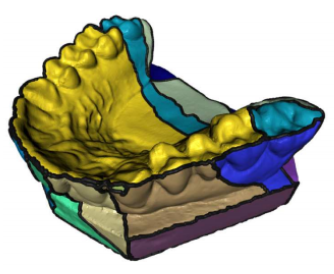
\includegraphics[width=0.8\textwidth]{teeth2}					
					\caption*{карманы}
				\end{subfigure}
				\begin{subfigure}{2in}
					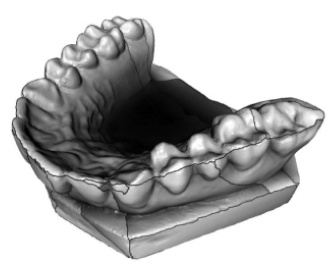
\includegraphics[width=0.8\textwidth]{teeth3}					
					\caption*{вогнутость}
				\end{subfigure}
				\caption{Алгоритм вычисления вогнутости фигуры}
				\label{teeth}
			\end{figure}
			\paragraph{Алгоритм} 
				Алгоритм вычисления вогнутости фигуры (рис.\,\ref{teeth}) заключается в следующем.
				Для объекта строятся мосты и карманы таким образом, чтобы между каждым караманом и мостом можно было установить взаимнооднозначную уникальную связь.
				Вогнутость $concave(x)$ подсчитывается как расстояние от точки $x$ кармана до соответсвующего моста $\beta_x$.
				$$concave(x) = distance(x, H_p) = distance(x, \beta_x)$$
				На правом изображении рисунка \ref{teeth} темный цвет означает более высокое значение меры вогнутости, светлый - низкое. 
	\section{Иерархия ограничивающих объемов}
		В задачах поиска пересечений с большим числом одновременно тестируемых объектов существует смысл определять, а какие объекты в данный момент времени в принципе могут пересечься и соответственно нужно тестировать.
		Для этого задача обнаружения колизий разбивается на две фазы: \emph{широкая фаза (broad phase)} и \emph{узкая фаза (narrow phase)}.
		Широкую фазу отвели на проверку возможности пересечения между телами, для этого достаточно вписать объект в некоторую простую фигуру, \emph{ограничивающий объем}, проверка на пересечение с которым будет занимать существенно меньше времени.
		В узкую фазу тестируется уже непосредственное пересечение пары объектов, в случае успеха широкой фазы для этих фигур.
	\subsection{Ограничивающие объемы}
		Теперь строго определим ограничивающий объем.\\
		\textbf{Ограничивающий объем} множества точек -- замкнутая фигура содержащая все точки этого множества.
		Существует много различных типов ограничивающих объемов с разной степенью ограничения и скорости тестирования, ниже на рис. \ref{bv_kianu} представлены некоторые из них.
		\begin{figure}[ht]
			\centering
			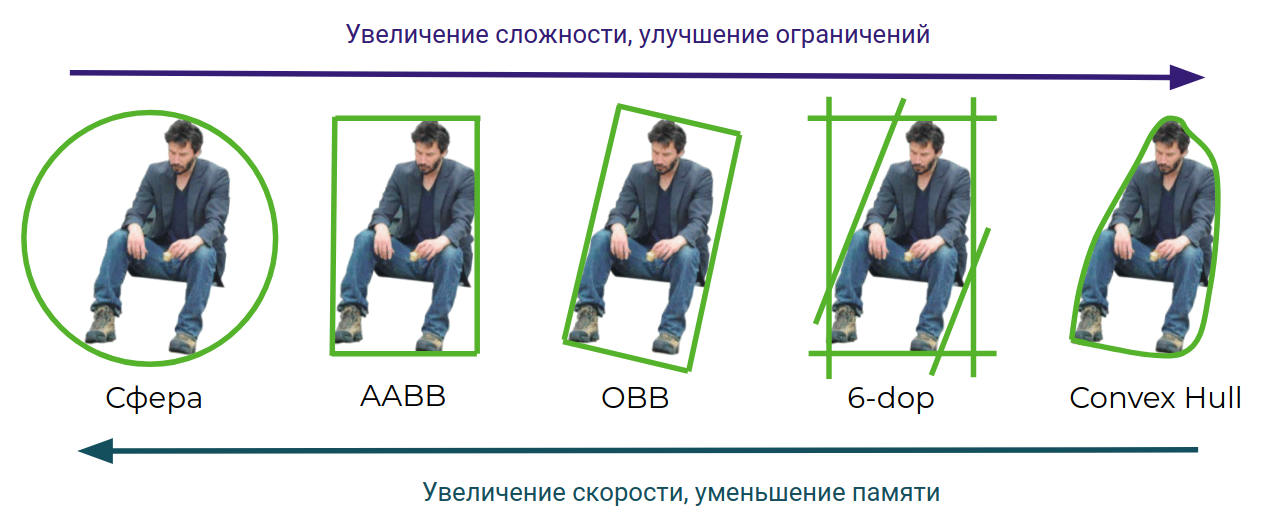
\includegraphics[width=0.9\textwidth]{bv_kianu}
			\caption{Примеры типов ограничивающих объемов}
			\label{bv_kianu}
		\end{figure}\\
		Чем сложнее объем - тем он лучше ограничивает тестируемое тело, тем медленее происходит проверка. \\
		Ограничивающие объемы могут стать полезны не только в широкой фазе, но и в узкой.
		Для этого вводится древовидная структура -- \emph{иерархия ограничивающих объемов (bvh)}.
		Некоторый объем ограничивающий объект или его часть называется \emph{узлом} иерархии.
		Сложный объект (root) делится на простые дочерние, причем на каждом уровне дети покрывают все вершины своего родителя
		(рис.\,\ref{bvhmodel}).
		\paragraph{Функция стоимости}
		Для вычисления сложности построенной иерархии ограничивающих объемов используется функция стоимости:
		\begin{equation*}
			T = N_vC_v + N_pC_P + N_uC_u, \text{ где }
		\end{equation*}
		\begin{equation*}			
			\begin{array}{ll}
				N_v\;\;\;-&\text{количество bv-пар, проверяемых на пересечение}\\
				C_v\;\;\;-&\text{стоимость проверки bv-пары на пересечение}\\
				N_p\;\;\;-&\text{количество тестируемых примитивов}\\
				C_p\;\;\;-&\text{стоимость теста примитивов}\\
				N_u\;\;\;-&\text{количество узлов для обновления}\\
				C_u\;\;\;-&\text{стоимость обновления узла}\\
			\end{array} 
		\end{equation*}
		\begin{figure}[ht]
			\centering
			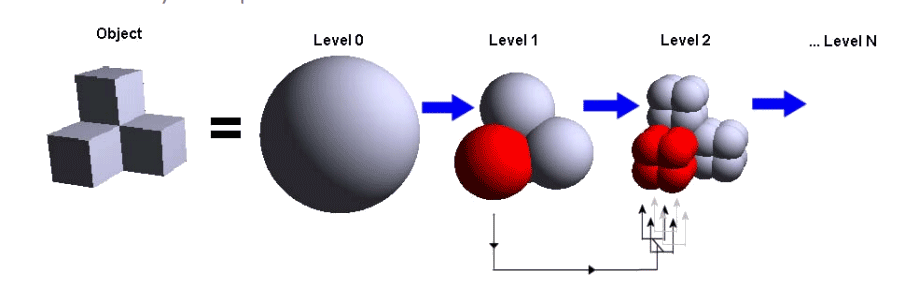
\includegraphics[width=0.9\textwidth]{bvhmodel}
			\caption{Модель иерархии сверху-вниз (top-down)}
			\label{bvhmodel}
		\end{figure}
		\subsection{Стратегии построения дерева иерархии}
			Как уже было сказанно в предыдущем параграфе BVH можно представить в виде дерева. 
			Эвристически показано что наиболее эффективное bvh-дерево для обнаружения пересечений является бинарным.
			При увеличении n-арности будет уменьшаться высота и время обхода, но возрастать временя на проверку узла.
			Существует несколько разных алгоритмов построения иерархии (рис.\,\ref{bvhcreate}).

			\paragraph{Стратегия сверху-вниз (Top-down)}
			Исходное множество ограничивается неким объемом (корень).
			До тех пор пока не выполнится условие, например не закончатся примитивы для разбиения, происходит рекурсивное разделение множества на два.
			Для эффективного выбора места разбиения можно использовать центр масс (рис.\,\ref{bvhcreate1}).\\
			\textbf{Достоинства}. Простота реализации, высокая скорость построения.\\
			\textbf{Недостатки}. В результате получается не всегда оптимальное решение.

			\paragraph{Стратегия снизу-вверх (Bottom-up)}
			Каждый примитив в множестве ограничиваются неким объемом (листья).
			Узлы объединяются под общими ограничивающими объемами, до тех пор пока не будет достигнут корень (рис.\,\ref{bvhcreate2}).\\
			\textbf{Достоинства}. Зачастую результат построения превосходит метод top-down.\\
			\textbf{Недостатки}. Скорость построения уступает предыдущей стратегии. Сложнее реализация.

			\paragraph{Стратегия вставками (Insertion)}
			В некой случайной последовательности для каждого объекта происходит поиск его места и вставка в изначально пустое дерево.
			Чем больше и дальше объект, тем он окажется выше (рис.\,\ref{bvhcreate3}).\\
			\textbf{Достоинства}. Удобен для динамических систем, высокая скорость обновления дерева.\\
			\textbf{Недостатки}. Дерево растет максимально медленно. Сложная реализация.

			\begin{figure}[ht]
				\centering
				\begin{subfigure}{1.5in}
					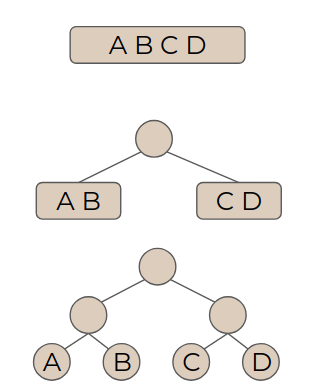
\includegraphics[width=\textwidth]{bvhcreate1}					
					\caption{top-down}
					\label{bvhcreate1}					
				\end{subfigure}
				\begin{subfigure}{1.5in}
					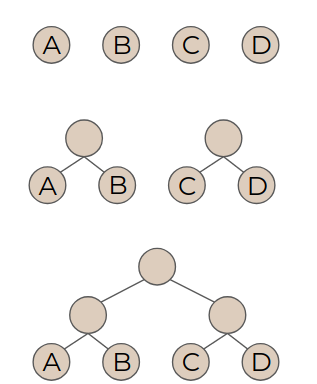
\includegraphics[width=\textwidth]{bvhcreate2}					
					\caption{bottom-up}
					\label{bvhcreate2}					
				\end{subfigure}
				\begin{subfigure}{1.5in}
					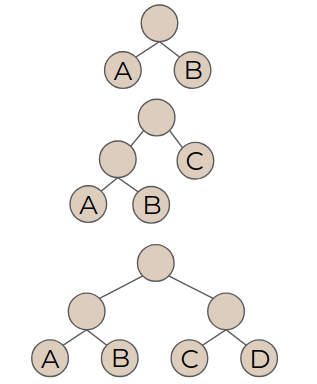
\includegraphics[width=\textwidth]{bvhcreate3}					
					\caption{insertion}
					\label{bvhcreate3}
			\end{subfigure}
				\caption{Стратегии построения bvh-дерева}
				\label{bvhcreate}
			\end{figure}

		\subsection{Стратегии обхода дерева иерархии}
			Существует два основных подхода в обходе bvh-деревьев. 
			\emph{Depth-first search (поиск в глубину)} -- самый широко используемый алгоритм в задачах обнаружения пересечений (рис.\,\ref{bvhtravers1}).
			\emph{Breadth-first search (поиск в ширину)} -- требует больше памяти, удобен для прерываемых систем поиска столкновений (рис.\,\ref{bvhtravers2}).
			
			Подходы приведенные выше не зависят от данных в структуре, а зависят только от самой структуры.
			Из-за чего эти методы также называют “слепыми”.
			С другой стороны есть \emph{Best-first search (поиск по наилучшему совпадению)} (рис.\,\ref{bvhtravers3}).
			Жадный алгоритм, который всегда перемещается к узлу наилучшему по какому-то заданному критерию, например по расстоянию до цели.
			
			\begin{figure}[ht]
				\centering
				\begin{subfigure}{2in}
					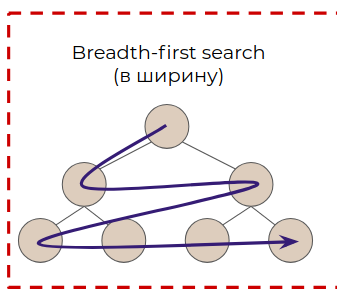
\includegraphics[width=\textwidth]{bvhtravers1}					
					\caption{}
					\label{bvhtravers1}					
				\end{subfigure}
				\begin{subfigure}{2in}
					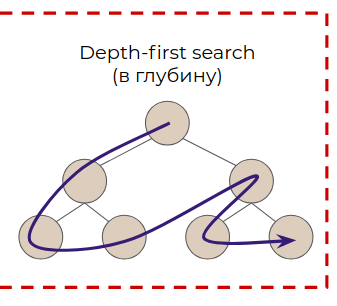
\includegraphics[width=\textwidth]{bvhtravers2}					
					\caption{}
					\label{bvhtravers2}					
				\end{subfigure}
				\begin{subfigure}{2in}
					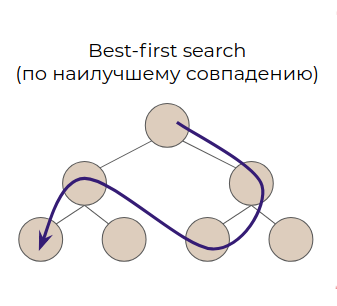
\includegraphics[width=\textwidth]{bvhtravers3}					
					\caption{}
					\label{bvhtravers3}
			\end{subfigure}
				\caption{Стратегии обхода bvh-дерева. Выделенные методы - “слепые”}
				\label{bvhtravers}
			\end{figure}

		\subsection{Использование BVH-дерева в задачах обнаружения пересечений}
			\paragraph{Суть алгоритма}
			В начале на пересечение тестируются корни двух объектов.
			Если корни пересеклись происходит рекурсивная проверка левого и правого дочернего поддерева на пересечение.
			В зависимости от выбранного метода обхода будет получаться разная производительность.
			Наиболее часто для задач обнаружения столкновений используется алгоритм поиска в глубину, как наиболее универсальный.
			\begin{figure}[ht]
				\centering
				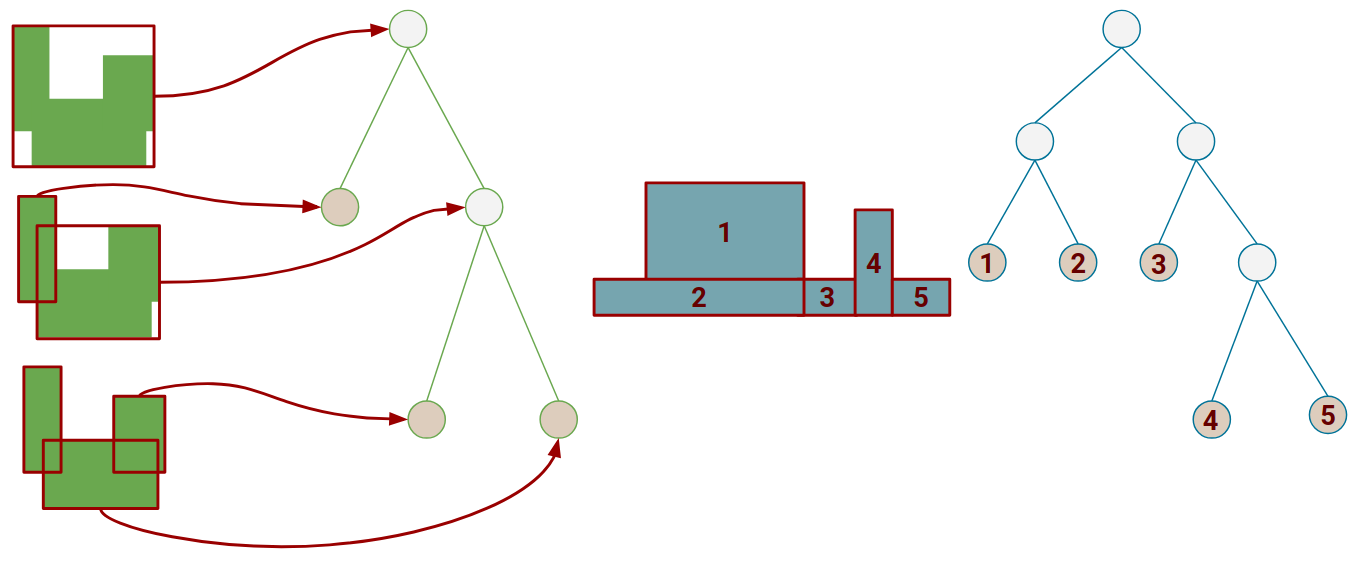
\includegraphics[width=\textwidth]{bvhcd}
				\caption{Алгоритм построения bvh-дерева по объекту}
			\end{figure}
	\newpage
	\section{Реализация алгоритма разбиения}
		Для реализации алгоритма приближенного разбиения была выбрана библиотека с открытым исходным кодом HACD, как наиболее близкая к статье Jyh-Ming Lien\cite{JMLien06} о выпуклой декомпозиции.
		\subsection{Инструменты}
			Я использовал:
			\begin{compactlist}
				\item ОС: Ubuntu 16.04
				\item Intel Core i5-6200U 2.3 MHz
				\item Графический редактор Blender 2.79b - для визуализации результата
				\item HACD - библиотека приближенной декомпозиции
				\item Библиотеки OBJLoader и OFFLoader для загрузки объектных файлов в программу
				\item Язык C++, std11
			\end{compactlist}
		\subsection{Алгоритм}
			На вход программа получает объектный файл в формате .off или .obj.\\
			Вызывается функция Scene::parseOFF() или Scene::parseOBJ(), которая создает Object obj и распарсивает объектный файл.
			После предварительной конфигурации вызывается функция obj->compute() и начинается процесс декомпозиции.
			В результате на выходе получается .off файл, который можно открыть в графическом редакторе Blender.
		\subsection{Результаты}
		Сравнение точной и приближенной декомпозиции:
		\begin{figure}[ht]
			\centering 
			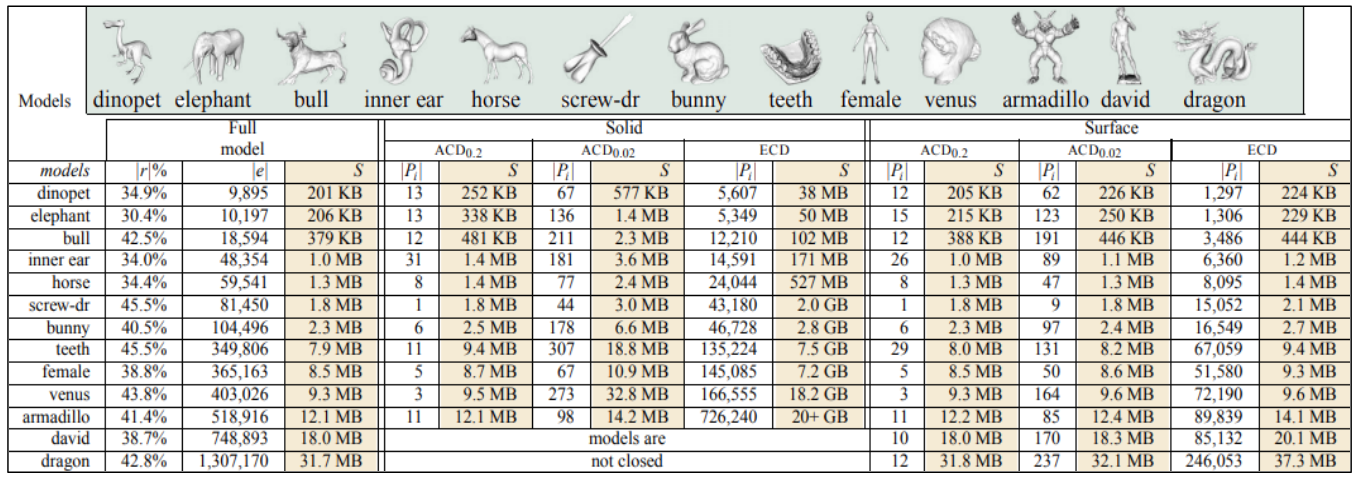
\includegraphics[width=\textwidth]{result}
			\caption{Таблица декомпозиции 14 моделей}
			\label{result}
		\end{figure}\\
		\noindent
		В таблице \ref{result}:\\
		$|r|\%$ - процент невыпуклости модели\\
		$|e|$ - число ребер модели\\
		$S$ - физический размер	модели \\
		$|P_i|$ - число компонент декомпозиции модели
		
		\newpage
		\begin{figure}[ht]
			\centering
			\begin{subfigure}{2in}
				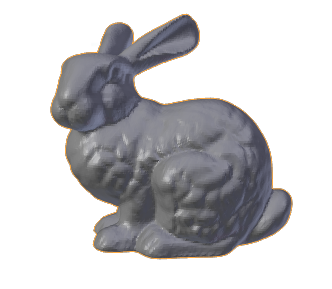
\includegraphics[width=\textwidth]{bunny}					
				\caption{исходный}
				\label{bunny1}					
			\end{subfigure}
			\begin{subfigure}{2in}
				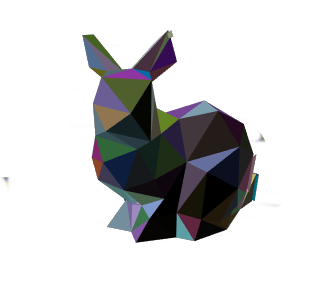
\includegraphics[width=\textwidth]{bunny_hacd200}					
				\caption{200 частей}
				\label{bunny2}					
			\end{subfigure}
			\begin{subfigure}{2in}
				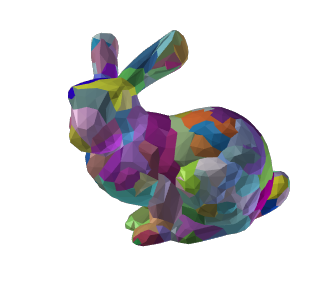
\includegraphics[width=\textwidth]{bunny_hacd3000}					
				\caption{3000 частей}
				\label{bunny3}
		\end{subfigure}
			\caption{Работа программы}
			\label{bunny}
		\end{figure}

		\paragraph{Время работы}
		Время декомпозиции при изменении параметра точности:
		\begin{compactlist}
			\item 10 частей - real 0m4.282s
			\item 200 частей - real 0m11.341s
			\item 3000 частей - real 0m43.883s
			\item 7611 частей - real 36m40.183s
		\end{compactlist}
	\section{Заключение}
		Подведем итоги.
		Были рассмотрены основные методы декомпозиции, такие как триангуляция Делоне, тетрайдаризация, методы точного и приблизительного разбиения.
		Приведены три возможных алгоритма решения NP-полной задачи о невозможности разбиения невыпуклых многогранников, такие как технология CSG, точки Штейнера, полигональный суп.
		Были сравнены оптимальные стратегии построения и обхода дерева иерархий ограничивающих объемов.
		Реализован алгоритм приближенного разбиения, работающий в связке с графическим редактором blender.
		
		После изучения темы было обнаружено, что приближенное разбиение с заранее выставленной точностью может решить большиство задач декомпозиции, при этом сильно сэкономив на вычислительные ресурсах и времени разбиения.
		
	

\newpage
\begin{thebibliography}{00}

	\bibitem{RTCD}
	\textbf{Christer Ericson}.
	\emph{Real-Time Collision Detection}.
	Sony Computer Entertainment, Santa Monica, USA,
	December, 2004.

	\bibitem{EhmLi02}
	\textbf{Stephen A. Ehmann, Ming C. Li}.
	\emph{Accurate and Fast Proximity Queries Between Polyhedra Using Convex Surface Decomposition}.
	University of North Carolina, Chapel Hill,
	July, 2002.

	\bibitem{RupSei92}
	\textbf{J.Ruppert, R.Seidel}.
	\emph{On the Difficulty of Triangulating Three-Dimensional Nonconvex Polyhedra}.
	University of California, Berkele, 
	December, 1992 

	\bibitem{Quinlan94}
	\textbf{S. Quinlan}.
	\emph{Efficient Distance Computation between Non-Convex Objects}.
	Stanford University,
	May, 1994

	\bibitem{JMLien06} 
	\textbf{Jyh-Ming Lien}.
	\emph{Approximate Convex Decomposition of Polyhedra}.
	2006 

	\bibitem{ZLK06}
	\textbf{Xinyu Zhang, Minkyoung Lee, Young J. Kim}.
	\emph{Interactive Continuous Collision Detection for Non-Convex Polyhedra}.
	2006

	\bibitem{RJA18}
	\textbf{Rui S.V. Rodrigues, José F.M. Morgado, Abel J.P. Gomes}.
	\emph{Part-Based Mesh Segmentation: A Survey}.
	2018

	\bibitem{Manzke}
	\textbf{Michael Manzke}.
	\emph{Bounding Volume Hierarchies presentation}.
	The University of Dublin,
	2015
	
	\bibitem{cshape2d}
	Visualization of Delaunay triangulation computed via the convex hull of lifted 2D points to a 3D paraboloid
		- \href{https://github.com/jmlien/cshape2d}{https://github.com/jmlien/cshape2d}

	\bibitem{img_delone}
	Delaunay image triangulatin - 
	\href{https://github.com/snorpey/triangulate-image}{https://github.com/snorpey/triangulate-image}

	\bibitem{acd2d}
	Approximate Convex Decomposition of Polygons - 
	\href{https://github.com/jmlien/acd2d}
	{https://github.com/jmlien/acd2d}

	\bibitem{bmesh}
	Bounding Mesh Library -
	\href{https://github.com/gaschler/bounding-mesh}{https://github.com/gaschler/bounding-mesh}

	\bibitem{HACD}
	HACD Library -
	\href{https://github.com/kmammou/v-hacd}{https://github.com/kmammou/v-hacd}


\end{thebibliography}
	
\end{document}